\section{Regularization Techniques}

        Commonly used neural network regularization techniques are explained in this section in details.

        \begin{itemize}

            \item \textbf{Data Augmentation}

                Data augmentation is artificially boosting the diversity and number of training examples by performing random transformations to existing images to create a set of new variants without altering the meaning of the data.
                Flipping, rotating, adding noise are the some of the commonly used data augmentation techniques.

                Data augmentation is used to prevent overfitting and especially useful when the training dataset is relatively small.
                While some augmentation increases the robustness of the algorithm, irrelevant transformations might make the task hard to learn, and adding new data to the training set will increase the model complexity and reqiured time to build the model.

            \item \textbf{Dropout}

                Overfitting is a common problem which is not limited only deep neural networks but includes the different disciplines such as several supervised and unsupervised methods in machine learning.
                Neural networks can be used to create relation between their input and output to predict the newly added input with acceptible result.
                It can be said that there is an overfitting if the results are not good for the unknown test data but good for the training data.

                Feeding the neural network with more training data is the simplest way which can be tried to prevent overfitting.
                This may effective if the newly added training data bring about new features which may increase the representativeness of the model. On the other hand, more training data will require more training time because it increase the model complexity.
                Bootstrap aggregating is another method which increase the network success \cite{breiman1996bagging}.
                This method classify different subsets of the training data, and fit a model based on these subsets.

                \citet{srivastava2014dropout} said that feature vectors should be combined instead of a single feature detector in order to describe meaningful features.
                They found out that  individual feature detectors start to detect helpful features afte dropping units from the neural network randomly.

                \begin{figure}
    \centerline{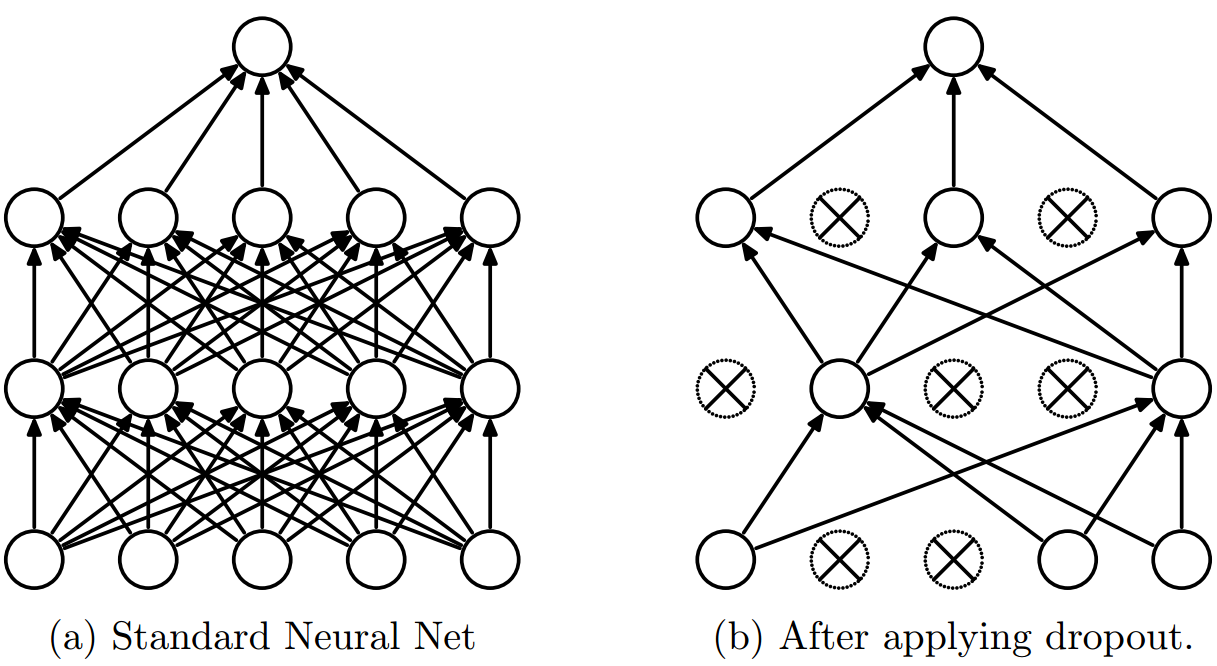
\includegraphics[width=1\columnwidth]{03-neural-networks-in-tumor-detection/figures/dropout.png}}
    \caption{ Dropout neural network model }
    \label{fig:dropout}
\end{figure}

                Dropout is a method of improvement aims to increase the performance of a neural network by reducing the overfitting \cite{srivastava2014dropout}.
                It's not only for CNNs but also all neural networks. At each training step, a new subset is excluded to improve the network's ability to generalize.
                The amount of exclusion is regulated by the dropout rate.
                Figure~\ref{figure:dropout} shows a regular neural network (a) and a thinned network by applying dropout (b).

            \item \textbf{Weight Decay}

                Weight decay is another technique used to prevent overfitting by adding a regularization term such as L1 or L2 to the loss function.
                L1 regularization is the sum of the absolute value of the weights and produces sparse weight matrices while L2 regularization is the sum of the squares of all the feature weights and make the calculation more computationally efficient.

                $$L_2\text{ regularization term} = ||\boldsymbol w||_2^2 = {w_1^2 + w_2^2 + ... + w_n^2}$$

                In L2 regularization, model complexity is dramatically affected by the outlier weights.

            \item \textbf{Early Stopping}

                Early stopping is a technique to reduce overfitting using the some part of the training data as a validation set.
                Training process does not include this data.
                If the error of the validation set reaches a certain amount, training is stopped at the training phase.
                It can be said that there is an overfitting exists in the current neural network for the training data.

                A significant point of eary stopping is selection of the validation set.
                It should represent the all data. It can be understood how well the model is generalizing beyond the training data.

        \end{itemize}

